\chapter{GARCH}
\label{GARCH}

\begin{figure}[h]
    \centering
    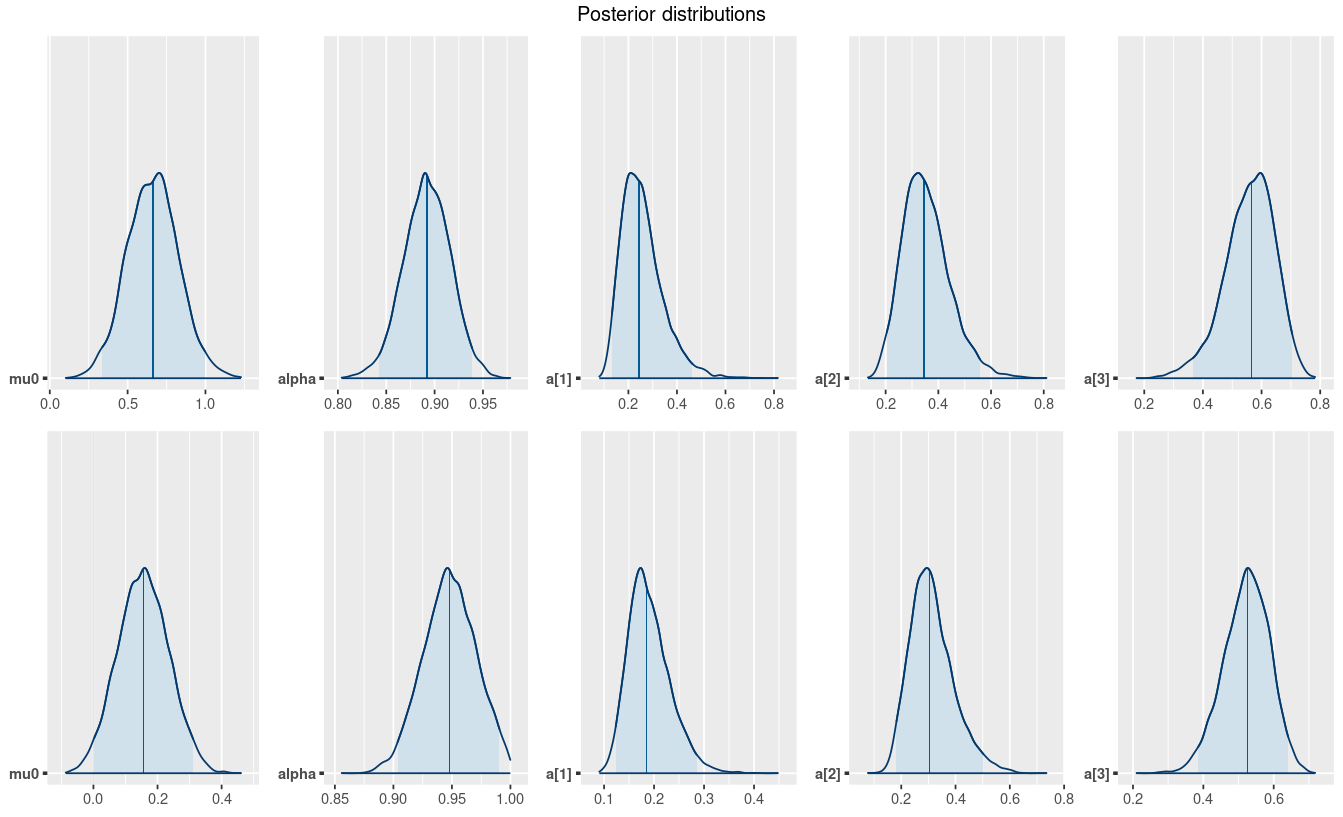
\includegraphics[width=\textwidth]{../Images/5-GARCH/posteriors.png}
    \caption{The image displays the posterior distributions of the parameters for the GARCH(1,1) model. The top line corresponds to the model used for GDP, while the bottom line corresponds to the model used for inflation.}
    \label{fig:GARCH_posteriors}
\end{figure}

\begin{figure}[h]
    \centering
    \begin{minipage}[t]{0.7\textwidth}
        \centering
        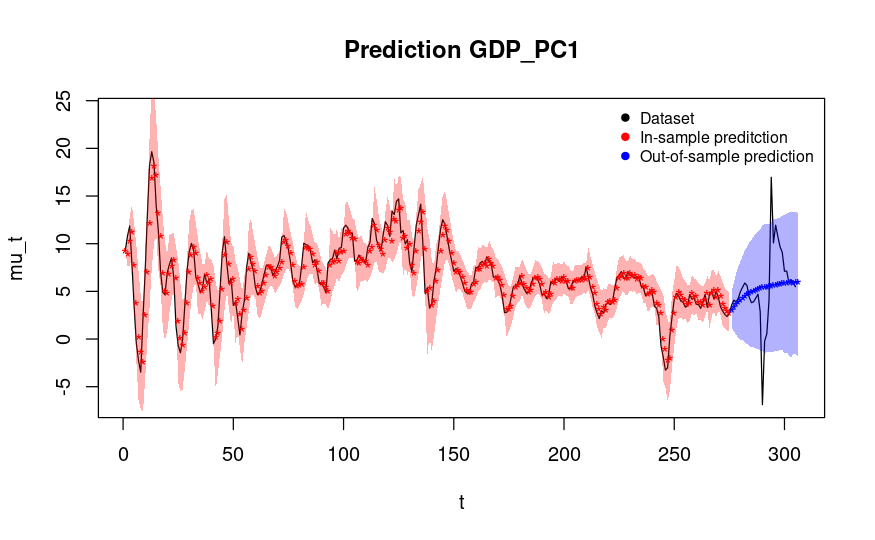
\includegraphics[width=\textwidth]{../Images/5-GARCH/gdp_prediction.png}
        \label{fig:GARCH_first}
    \end{minipage}
    \begin{minipage}[t]{0.7\textwidth}
        \centering
        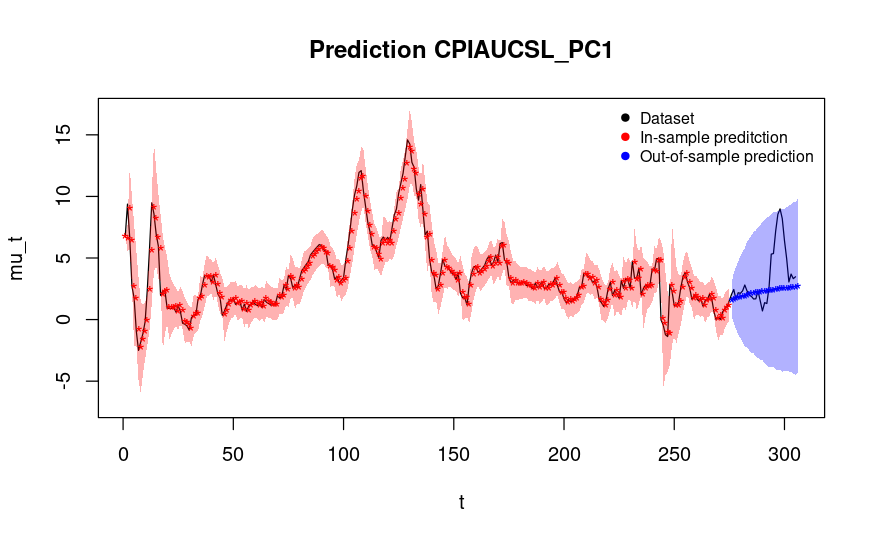
\includegraphics[width=\textwidth]{../Images/5-GARCH/infl_prediction.png}
        \label{fig:GARCH_second}
    \end{minipage}
    \caption{GARCH(1,1): In-sample and out-of-sample predictions}
    \label{fig:GARCH_combined}
\end{figure}